% \documentclass[table]{beamer}
\documentclass[table,handout]{beamer}
\setbeameroption{show notes}
% \setbeameroption{hide notes}
% \setbeameroption{show only notes}
\usepackage{varwidth}

\newif\ifhide
\newif\ifpost
\newif\ifhideclicker

% \hidetrue
% \hideclickertrue
% \posttrue

\newcommand{\whiteout}[1]{\textcolor{white}{#1}}
% \newcommand{\whiteoutbox}[1]{\fcolorbox{white}{white}{\parbox{\dimexpr \linewidth-2\fboxsep-2\fboxrule}{\whiteout{#1}}}}
% \newcommand{\notebox}[1]{\fcolorbox{blue}{white}{\parbox{\dimexpr \linewidth-2\fboxsep-2\fboxrule}{#1}}}
\newcommand{\whiteoutbox}[1]{\fcolorbox{white}{white}{\parbox{\linewidth}{\whiteout{#1}}}}
\newcommand{\notebox}[1]{\fcolorbox{blue}{white}{\parbox{\linewidth}{#1}}}
\newcommand{\blankbox}[1]{\phantom{\varwidth{\linewidth}\whiteoutbox{#1}\endvarwidth}}
\newcommand{\blank}[1]{\phantom{\varwidth{\linewidth}#1\endvarwidth}}

\ifhide%
    \newcommand{\hmask}[1]{\blank{#1}}%
\else%
    \newcommand{\hmask}[1]{#1}%
\fi

\ifhide%
    \newcommand{\wout}[1]{\whiteout{#1}}%
\else%
    \newcommand{\wout}[1]{#1}%
\fi

\ifhide%
    \newcommand{\hignore}[1]{}%
\else%
    \newcommand{\hignore}[1]{#1}%
\fi

\ifpost%
    \newcommand{\nopost}[1]{}%
\else%
    \newcommand{\nopost}[1]{#1}%
\fi

\ifhideclicker%
    \newcommand{\clickerslide}[1]{\stepcounter{clickerQuestionCounter}%
        \begin{frame}[t]
            \textcolor{blue}{Q \arabic{clickerQuestionCounter}:}
        \end{frame}}
\else%
    \newcommand{\clickerslide}[1]{#1}%
\fi

\ifhide%
    \newcommand{\hidebox}[1]{\blank{#1}}%
\else%
    \newcommand{\hidebox}[1]{\notebox{#1}}%
\fi

\ifhide%
    \newcommand{\wbox}[1]{\whiteoutbox{#1}}%
\else%
    \newcommand{\wbox}[1]{\notebox{#1}}%
\fi

\ifhide%
    \newcommand{\nbox}[1]{\blankbox{#1}}%
\else%
    \newcommand{\nbox}[1]{\notebox{#1}}%
\fi

\ifhideclicker%
    \newcommand{\clickeranswer}[1]{#1}%
\else%
    \ifhide%
        \newcommand{\clickeranswer}[1]{#1}%
    \else%
        \newcommand{\clickeranswer}[1]{\textbf{\textcolor{blue}{#1}}}%
    \fi
\fi

\usepackage{beamerthemesplit}
% \usetheme{boxes}
\usetheme{Malmoe}
\usecolortheme{seahorse}
% \usecolortheme{seagull}
\usepackage{ifthen}
\usepackage{xspace}
\usepackage{multirow}
\usepackage{multicol}
\usepackage{booktabs}
\usepackage{xcolor}
\usepackage{wasysym}
\usepackage{comment}
\usepackage{hyperref}
\hypersetup{pdfborder={0 0 0}, colorlinks=true, urlcolor=blue, linkcolor=blue, citecolor=blue}
\usepackage{changepage}
\usepackage[compatibility=false]{caption}
\captionsetup[figure]{font=scriptsize, labelformat=empty, textformat=simple, justification=centering, skip=2pt}
\usepackage{tikz}
\usetikzlibrary{trees,calc,backgrounds}

\usepackage[bibstyle=joaks-slides,maxcitenames=3,mincitenames=1,backend=biber]{biblatex}

\newrobustcmd*{\shortfullcite}{\AtNextCite{\renewbibmacro{title}{}\renewbibmacro{in:}{}\renewbibmacro{number}{}}\fullcite}

\newrobustcmd*{\footlessfullcite}{\AtNextCite{\renewbibmacro{title}{}\renewbibmacro{in:}{}}\footfullcite}

% Make all footnotes smaller
% \renewcommand{\footnotesize}{\scriptsize}

\definecolor{myGray}{gray}{0.9}
\colorlet{rowred}{red!30!white}

\setbeamertemplate{blocks}[rounded][shadow=true]

\setbeamercolor{defaultcolor}{bg=structure!30!normal text.bg,fg=black}
\setbeamercolor{block body}{bg=structure!30!normal text.bg,fg=black}
\setbeamercolor{block title}{bg=structure!50!normal text.bg,fg=black}

\newenvironment<>{varblock}[2][\textwidth]{%
  \setlength{\textwidth}{#1}
  \begin{actionenv}#3%
    \def\insertblocktitle{#2}%
    \par%
    \usebeamertemplate{block begin}}
  {\par%
    \usebeamertemplate{block end}%
  \end{actionenv}}

\newenvironment{displaybox}[1][\textwidth]
{
    \centerline\bgroup\hfill
    \begin{beamerboxesrounded}[lower=defaultcolor,shadow=true,width=#1]{}
}
{
    \end{beamerboxesrounded}\hfill\egroup
}

\newenvironment{onlinebox}[1][4cm]
{
    \newbox\mybox
    \newdimen\myboxht
    \setbox\mybox\hbox\bgroup%
        \begin{beamerboxesrounded}[lower=defaultcolor,shadow=true,width=#1]{}
    \centering
}
{
    \end{beamerboxesrounded}\egroup
    \myboxht\ht\mybox
    \raisebox{-0.25\myboxht}{\usebox\mybox}\hspace{2pt}
}

\newenvironment{mydescription}{
    \begin{description}
        \setlength{\leftskip}{-1.5cm}}
    {\end{description}}

\newenvironment{myitemize}{
    \begin{itemize}
        \setlength{\leftskip}{-.3cm}}
    {\end{itemize}}

% footnote without a marker
\newcommand\barefootnote[1]{%
  \begingroup
  \renewcommand\thefootnote{}\footnote{#1}%
  \addtocounter{footnote}{-1}%
  \endgroup
}

% define formatting for footer
\newcommand{\myfootline}{%
    {\it
    \insertshorttitle
    \hspace*{\fill} 
    \insertshortauthor, \insertshortinstitute
    % \ifx\insertsubtitle\@empty\else, \insertshortsubtitle\fi
    \hspace*{\fill}
    \insertframenumber/\inserttotalframenumber}}

% set up footer
\setbeamertemplate{footline}{%
    \usebeamerfont{structure}
    \begin{beamercolorbox}[wd=\paperwidth,ht=2.25ex,dp=1ex]{frametitle}%
        % \Tiny\hspace*{4mm}\myfootline\hspace{4mm}
        \tiny\hspace*{4mm}\myfootline\hspace{4mm}
    \end{beamercolorbox}}

% remove navigation bar
\beamertemplatenavigationsymbolsempty

\makeatletter
    \newenvironment{noheadline}{
        \setbeamertemplate{headline}[default]
        \def\beamer@entrycode{\vspace*{-\headheight}}
    }{}
\makeatother

\newcounter{clickerQuestionCounter}
\ifhideclicker%
\newenvironment{clickerquestion}
{ \stepcounter{clickerQuestionCounter}
  \begin{enumerate}[Q \arabic{clickerQuestionCounter}:]\color{white} }
{ \end{enumerate} }
\else%
\newenvironment{clickerquestion}
{ \stepcounter{clickerQuestionCounter}
  \begin{enumerate}[Q \arabic{clickerQuestionCounter}:] }
{ \end{enumerate} }
\fi

\ifhideclicker%
\newenvironment{clickeroptions}
{ \begin{enumerate}[\begingroup\color{white} 1)\endgroup]\color{white} }
{ \end{enumerate} }
\else%
\newenvironment{clickeroptions}
{ \begin{enumerate}[\begingroup\color{red} 1)\endgroup] }
{ \end{enumerate} }
\fi


\tikzstyle{centered} = [align=center, text centered, font=\sffamily\bfseries]
\tikzstyle{skip} = [centered, inner sep=0pt, fill]
\tikzstyle{empty} = [centered, inner sep=0pt]
\tikzstyle{inode} = [centered, circle, minimum width=4pt, fill=black, inner sep=0pt]
\tikzstyle{tnode} = [centered, circle, inner sep=1pt]
\tikzset{
  % edge styles
  level distance=10mm,
  mate/.style={edge from parent/.style={draw,distance=3pt}},
  mleft/.style={grow=left, level distance=10mm, edge from parent path={(\tikzparentnode.west)--(\tikzchildnode.east)}},
  mright/.style={grow=right, level distance=10mm, edge from parent path={(\tikzparentnode.east)--(\tikzchildnode.west)}},
  % node styles
  male/.style={rectangle,minimum size=4mm,fill=gray!80},
  female/.style={circle,minimum size=4mm,fill=gray!80},
  amale/.style={male,fill=red},
  afemale/.style={female,fill=red},
}

\newcommand{\highlight}[1]{\textcolor{violet}{\textit{\textbf{#1}}}}
\newcommand{\super}[1]{\ensuremath{^{\textrm{\sffamily #1}}}}
\newcommand{\sub}[1]{\ensuremath{_{\textrm{\sffamily #1}}}}
\newcommand{\dC}{\ensuremath{^\circ{\textrm{C}}}}
\newcommand{\tb}{\hspace{2em}}
\providecommand{\e}[1]{\ensuremath{\times 10^{#1}}}
\newcommand{\myHangIndent}{\hangindent=5mm}

\newcommand{\spp}[1]{\textit{#1}}

\newcommand\mybullet{\leavevmode%
\usebeamertemplate{itemize item}\hspace{.5em}}

\makeatletter
\newcommand*{\rom}[1]{\expandafter\@slowromancap\romannumeral #1@}
\makeatother

\newcommand{\blankslide}{{\setbeamercolor{background canvas}{bg=black}
\setbeamercolor{whitetext}{fg=white}
\begin{frame}<handout:0>[plain]
\end{frame}}}

\newcommand{\whiteslide}{
\begin{frame}<handout:0>[plain]
\end{frame}}

\newcommand{\f}[1]{\ensuremath{F_{#1}}}
\newcommand{\x}[1]{X\ensuremath{^{#1}}}
\newcommand{\y}[1]{Y\ensuremath{^{#1}}}

% Population growth macros
\newcommand{\popsize}[1]{\ensuremath{N_{#1}}}
\newcommand{\popgrowthratediscrete}[1]{\ensuremath{\lambda_{#1}}}
\newcommand{\popgrowthrate}[1]{\ensuremath{r_{#1}}}
\newcommand{\ptime}{\ensuremath{t}\xspace}

\tikzset{hide on/.code={\only<#1>{\color{white}}}}
\tikzset{
    invisible/.style={opacity=0},
    visible on/.style={alt={#1{}{invisible}}},
    alt/.code args={<#1>#2#3}{%
        \alt<#1>{\pgfkeysalso{#2}}{\pgfkeysalso{#3}}
        % \pgfkeysalso doesn't change the path
    },
}

% \bibliography{../bib/references}
\bibliography{references}
\author[J.\ Oaks]{
    %Jamie R.\ Oaks\inst{1}
    Jamie R.\ Oaks
}
\institute[BIOL 180]{
    \inst{}%
        BIOL 180: Introductory Biology
}



\title[Professional Development I]{Professional Development I: Study skills}
% \date{\today}
\date{March 31, 2015}

\begin{document}

\begin{noheadline}
\maketitle
\end{noheadline}

\nopost{
\begin{noheadline}
\begin{frame}[c]
    \vspace{-6mm}
    \begin{center} 
        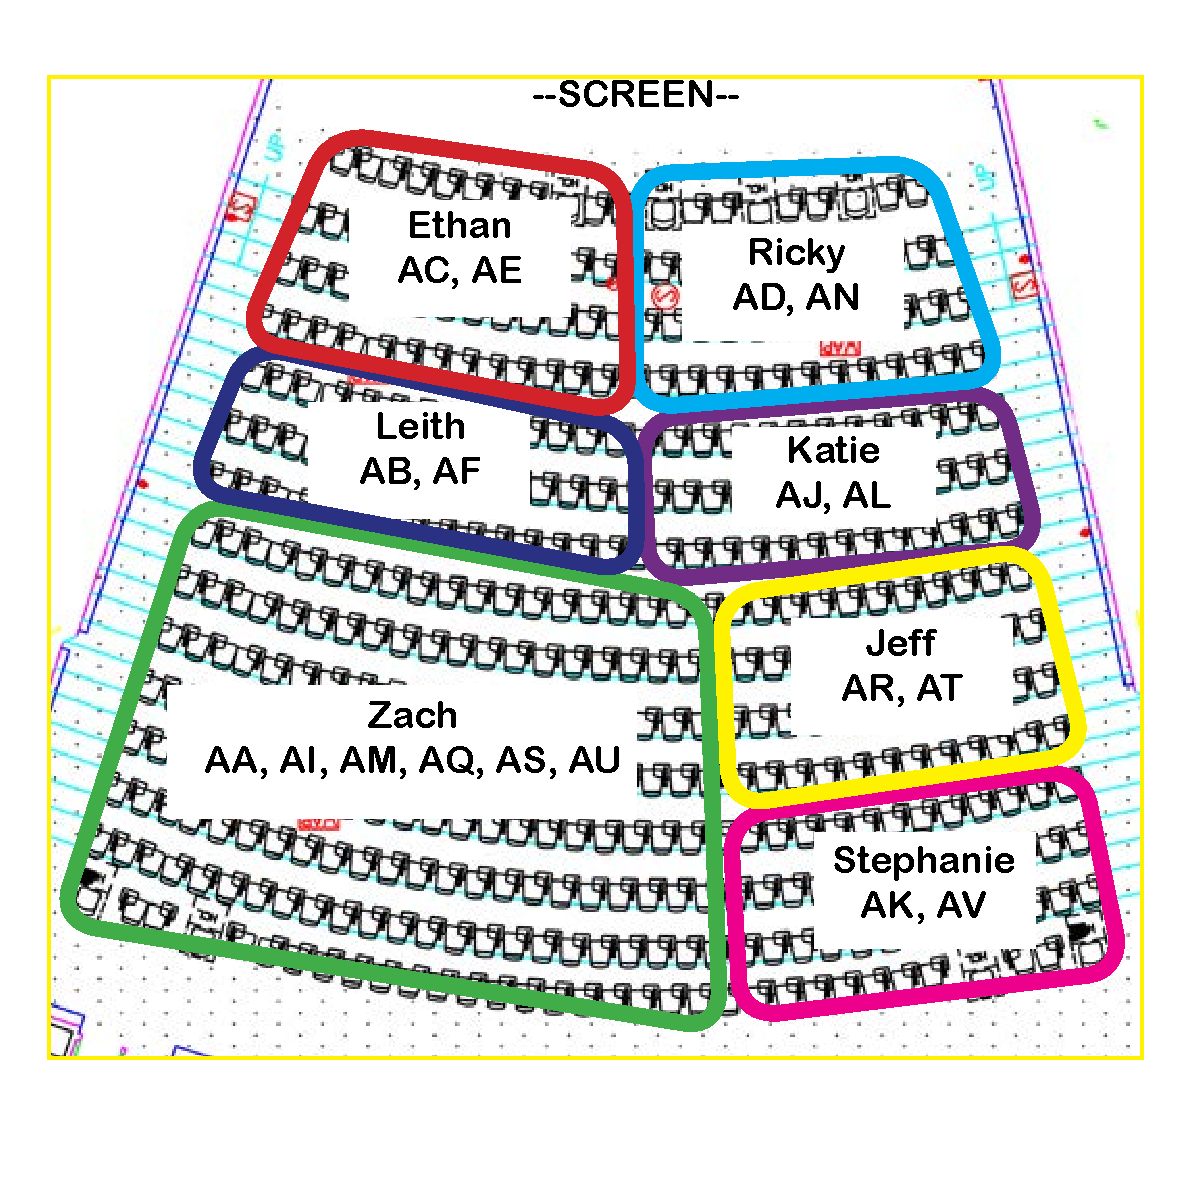
\includegraphics[height=1.3\textheight]{../images/seating-chart.pdf}
    \end{center}
\end{frame}
\end{noheadline}
}

\begin{noheadline}
\begin{frame}
\frametitle{Today's issues:}
\tableofcontents[subsectionstyle=hide]
\end{frame}
\end{noheadline}

\section{What does it mean to be a DAWG?}

\begin{noheadline}
\begin{frame}
    \frametitle{Being a \highlight{DAWG}}

    \begin{itemize}[<+->]
        \item Olympic games, Berlin, 1936
        \item UW men's 8-oar rowing team won Olympic trials
        \item U.S.O.C.\ gave UW crew 1 week to raise \$5000 to pay for trip to
            Germany
        \item Despite being top qualifiers, they were given the worst lane
        \begin{itemize}
            \item Who got the two best lanes?
            \item Cost UW two boat lengths
        \end{itemize}
        \item The starter gave Germany and Italy unfair advantage (1.5 strokes)
        \item UW stroke was sick---lost 14 lbs; almost passed out
        \item UW lane was next to the stands of 70,000 German fans---the rowers
            couldn't hear the cox
        \item Hitler, G\"{o}ring, and Goebbels were watching
    \end{itemize}
\end{frame}
\end{noheadline}

\begin{noheadline}
\begin{frame}
    \frametitle{Being a \highlight{DAWG}}
    \includegraphics<1| handout:1>[page=1,width=\linewidth]{./uw-row-win.png}
\end{frame}
\end{noheadline}

\begin{noheadline}
\begin{frame}
    \frametitle{Being a \highlight{DAWG}}
    \includegraphics<1| handout:1>[page=1,width=\linewidth]{./uw-row-team.png}
\end{frame}
\end{noheadline}

\begin{noheadline}
\begin{frame}
    \frametitle{Being a \highlight{DAWG}}
    \begin{itemize}[<+->]
        \item You will forget almost all the content you'll be learning in BIO 180
        \item We want you to remember\ldots
            \begin{itemize}
                \item How to conduct yourself as a professional
                \item How to study
                \item How to be a \highlight{DAWG}!
            \end{itemize}
    \end{itemize}
\end{frame}
\end{noheadline}

\section{Professional correspondence}

\begin{noheadline}
\begin{frame}
    \frametitle{Professional correspondence: E-mail}

    \uncover<2->{
    Date: \\
    To: \\
    From: \\
    RE:
    }

    \uncover<3->{
    \bigskip
    Dear Dr.\ Freeman:
    }

    \uncover<4->{
    \smallskip
    I was interested in the example from class today about \ldots
    }

    \uncover<5->{
    \bigskip
    Sincerely,

    \smallskip
    Jane Doe
    }

    \uncover<6->{
    \bigskip
    Jane Doe, Pre-major, Class of 2018 \\
    Dream Project Volunteer \\
    University of Washington \\
    jdoe@uw.edu
    }
\end{frame}
\end{noheadline}

\begin{noheadline}
\begin{frame}
    \frametitle{Professional correspondence: Course discussion forum}

\end{frame}
\end{noheadline}

\section{How should you study for this course?}

\begin{noheadline}
\begin{frame}
    \frametitle{How should you study for this course?}
    \begin{itemize}%[<+->]
        \item BIO 180/200/220 exams are short answer (2--3 sentences, making
            graphs, labeling, some single-word)
        \item Consider what it takes to excel on a multiple-choice test versus
            a short-answer exam. How does your level of understanding compare?
            \wbox{You have to be able to synthesize the correct answer, rather
                than simply identify it.}
        \item Why is it extremely common for instructors to hear, ``I
            understood the material so well, but I got a 47 on the exam?''
            \wbox{Because students are in the habit of only learning at the
                lower-level of Bloom's hierarchy}
    \end{itemize}

\end{frame}
\end{noheadline}

\begin{noheadline}
\begin{frame}[t]
    \begin{adjustwidth}{-1.5em}{-1.5em}
    \vspace{-2mm}
    \centerline{
    \includegraphics<1->[page=1,width=0.85\linewidth]{./bloom.png}
    }

    \vspace{-1mm}
    \begin{uncoverenv}<2->
    \begin{block}{\small\it Weighted Bloom's Index (WBI):}
    \begin{columns}
        \column{0.35\textwidth}
            \small
            \begin{align*}
                \small
                &WBI = \frac{\sum_{i}^{n} (P_i \times B)}{
                    T \times 6} \times 100 \\
            \end{align*}
        \column{0.5\textwidth}
            \vspace{-4.5mm}
            {\footnotesize
            \begin{align*}
                &n = \textrm{Number of questions on exam} \\
                &P_i = \textrm{Point value of question $i$}\\
                &B = \textrm{Bloom level}\\
                &T = \textrm{Total points on the exam}
            \end{align*}
            }
            \vspace{-6.5mm}
    \end{columns}
    \end{block}
    \end{uncoverenv}

    % \vspace{1mm}
    \begin{uncoverenv}<3->
    \centerline{
    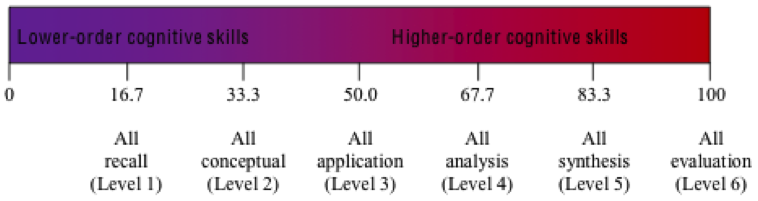
\includegraphics[page=1,width=0.75\linewidth]{./bloom-scale.png}
    }
    \end{uncoverenv}
    \end{adjustwidth}
\end{frame}
\end{noheadline}

\begin{noheadline}
\begin{frame}
    \centerline{
    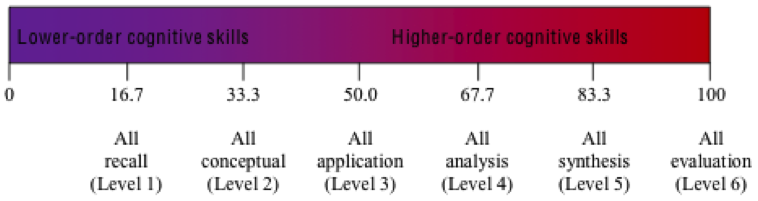
\includegraphics[width=0.75\linewidth]{./bloom-scale.png}}
    
    \vspace{2mm}
    \centerline{
    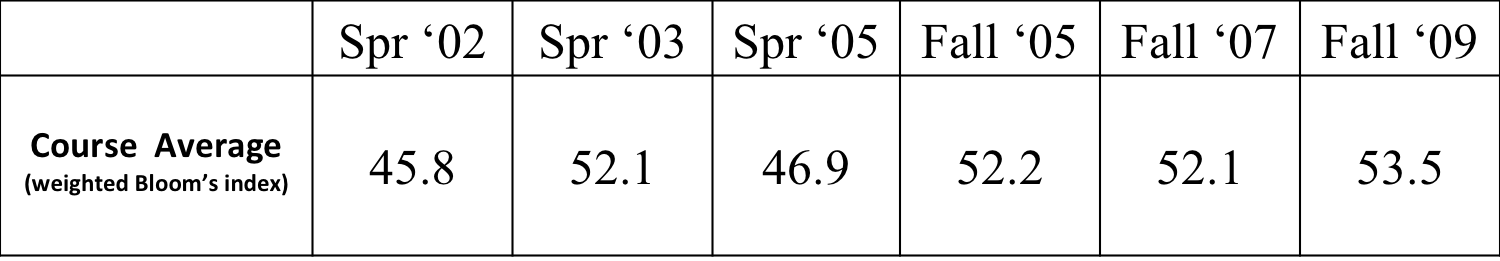
\includegraphics[width=\linewidth]{./bloom-data.png}}
    \begin{clickerquestion}
        \item What do these data tell you about the exams?
        \begin{clickeroptions}
            \item You can excel in this course by memorizing content
            \item \clickeranswer{On average, questions are at the application level}
            \item Most exam questions are of the ``plug and chug'' variety
            \item \clickeranswer{Over this period, the Bloom's level appears stable or increasing slightly}
        \end{clickeroptions}
    \end{clickerquestion}
\end{frame}
\end{noheadline}

\begin{noheadline}
\begin{frame}
    \begin{clickerquestion}
        \item According to education research, which of the following
            techniques is most effective?
        \begin{clickeroptions}
            \item Going over lecture notes and/or making outlines from them
            \item Highlighting the textbook
            \item \clickeranswer{Testing your understanding with exam-like
                    questions}
            \item Asking a tutor to go over concepts you don't understand
            \item \clickeranswer{Explaining concepts to members of a study
                    group, and having them them challenge you with questions}
        \end{clickeroptions}
    \end{clickerquestion}
\end{frame}
\end{noheadline}

\begin{noheadline}
\begin{frame}
    \frametitle{How should you study for this course?}
    \begin{itemize}[<+->]
        \item To excel in a college course, instructors tell students to budget
            $\approx$3 hours of studying for every hour of class
        \item BIO 180 students, on-average spend about 8 hours per week studying
            for the course
            \begin{itemize}
                \item How does this compare to the ``recommended dosage?''
                \item What is the best way to budget the time required?
            \end{itemize}
    \end{itemize}
\end{frame}
\end{noheadline}

\begin{noheadline}
\begin{frame}
    \frametitle{How should you study for this course?}
    Student quotes I: What is your frame of mind coming into this course? \\

    \uncover<2->{
    \begin{itemize}
        \item ``Do NOT stick with old styles of studying that don't work
            anymore. I used to be a flash card learner---now I'm a flow chart
            learner.''

        \item Why is it so difficult for students to change the way they study,
            in response to new demands?
            \wbox{Because, for 12+ years, they have mastered how to excel in
                school; that's why they are at UW. But now you are in a new
                learning environment.}
    \end{itemize}
    }
\end{frame}
\end{noheadline}

\begin{noheadline}
\begin{frame}
    \frametitle{How should you study for this course?}
    Student quotes II: What resources do you have available? \\

    \uncover<2->{
    \begin{itemize}
        \item ``Use the TA office hours and Tribeta office hours. Help the
            other students there---it will reinforce what you know and
            highlight what you don't understand.''

        \item ``I meet with a Tribeta tutor every week. She's an MCD major and
            works in a lab, and for each topic she asks me questions relevant
            to her research. This makes me apply the concepts from class in a
            new way.''
        \item In each quote above, underline the words that you find most
            important
    \end{itemize}
    }
\end{frame}
\end{noheadline}

\begin{noheadline}
\begin{frame}
    \frametitle{How should you study for this course?}
    Student quotes III: What strategies should you bring to your studying? \\

    \uncover<2->{
    \begin{itemize}
        \item ``Really focus on linking the ideas among lectures---synthesize the ideas.''
        \item ``Understand the material the day of---DO NOT WAIT.''
        \item In terms of the science of learning, WHY are these statements
            good advice? \\
        \wbox{1. Higher-level understanding (Bloom)! 2. Biology, and learning
            in general (think Bloom), is inherently cumulative.}
    \end{itemize}
    }
\end{frame}
\end{noheadline}

\begin{noheadline}
\begin{frame}
    \frametitle{How should you study for this course?}
    Student quotes IV: How should your study group operate? \\

    \uncover<2->{
    \begin{itemize}
        % \item ``Draw out schematics, with study partners. We made tons of
        %     pictures on a big whiteboard, explaining things to each other and
        %     making up mnemonics to remember key terms and processes.''
        \item ``We made big flow charts on a whiteboard---first from memory, and
            then correcting and completing them from our notes. This helped us
            diagnose gaps in our understanding.''
        % \item ``We meet in a group, sometimes via Skype for people who commute.
        %     We discuss concepts from lecture, quiz each other, and do the study
        %     questions and discuss the answers and grade each other before
        %     looking at the key.''
        % \item ``Our group does the study questions, and then we discuss
        %     everything around the topic of each question. For example with the
        %     RNA polymerase question, we discussed everything else that was
        %     going on at the start of transcription.''
        \item ``I can't meet with a study group because of my schedule, so I
            re-read the text to make sure all the key concepts are fresh. Then
            to diagnose what I don't understand, I teach the stuff to friends
            and my girlfriend, and they ask me questions.''
        % \item ``Every night, a study partner and I do the reading quiz
        %     questions at the same time, but in different rooms. We call out to
        %     ask each other things and explain the questions back and forth. If
        %     neither of us understands one, then we work through it. We also go
        %     over the clicker questions, and make sure we can explain why the
        %     right answer is right AND why the wrong answers are wrong.''
    \end{itemize}}
\end{frame}
\end{noheadline}

\begin{noheadline}
\begin{frame}
    \frametitle{How should you study for this course?}
    Student quotes V: How should you prepare for exams? \\

    \uncover<2->{
    \begin{itemize}
        \item ``When reviewing for the exam, focus on the slides.''
        \item ``We start meeting two weeks before exam. We do the study
            questions without the key, explaining our answers to each other and
            catching misconceptions. We also teach everything to each other
            using a big whiteboard---it's super important to draw things out a
            bunch of times.''
        \item When is two weeks before the first exam?
            \wbox{This Friday!!}
    \end{itemize}}
\end{frame}
\end{noheadline}

\begin{noheadline}
\begin{frame}
    \frametitle{GO \highlight{DAWGS}!!}
    \includegraphics<1| handout:1>[page=1,width=\linewidth]{./uw-row-win.png}
\end{frame}
\end{noheadline}

\end{document}


